\documentclass[a4paper,12pt]{report}
\usepackage[T2A]{fontenc}
\usepackage[utf8]{inputenc}
\usepackage[english,russian]{babel}
\usepackage{graphicx}
\usepackage{wrapfig}
\usepackage{mathtext} 				% русские буквы в фомулах
\usepackage{amsmath,amsfonts,amssymb,amsthm,mathtools} % AMS
\usepackage{icomma} % "Умная" запятая: $0,2$ --- число, $0, 2$ --- перечисление
\usepackage{capt-of}
\usepackage{appendix}
\usepackage{multirow}
\usepackage{hyperref}
\usepackage{floatrow}
\usepackage[left=2cm,right=2cm,
    top=2cm,bottom=2cm,bindingoffset=0cm]{geometry}
\usepackage{multicol} % Несколько колонок
\usepackage{gensymb}
\title{Отчёт по лабораторной работе №23

Изучение электропроводности и определение удельного сопротивления полупроводников}
\author{Богатова Е.}
\date{\today}

\begin{document}

\maketitle
\section*{1. Экспериментальная установка}

\begin{figure}[H]
    \centering	
    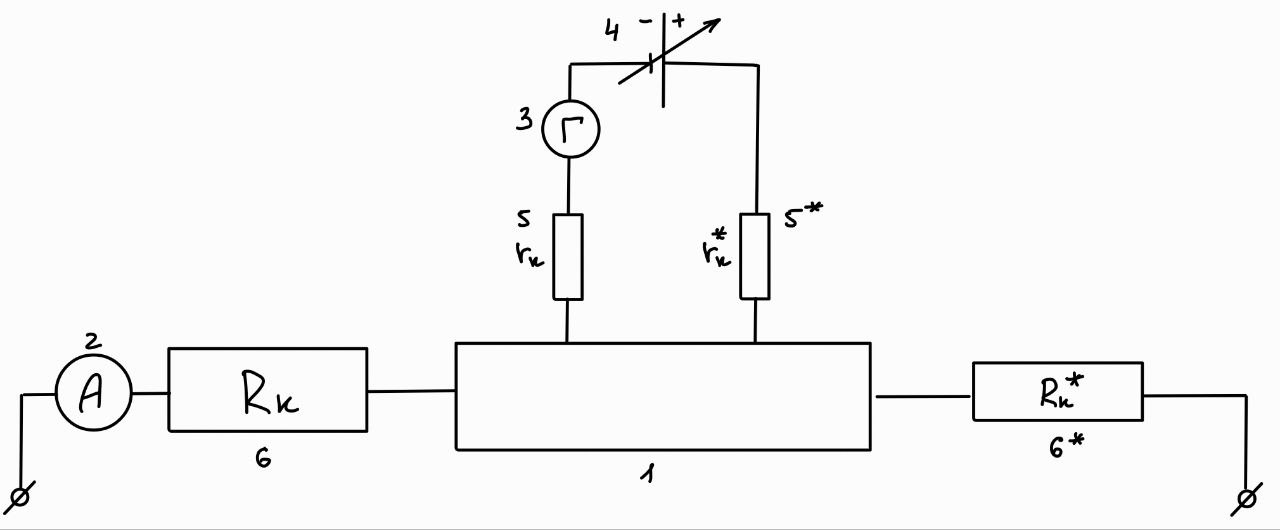
\includegraphics[width=0.87\textwidth]{ustanovka.jpg}
    \caption{Схема экспериментальной установки}
    \label{ustanovka}
\end{figure}

Для измерения сопротивления используется двухзондовый метод. На торцевые части полупроводникового образца наносятся металлические контакты, и образец в торцевых частях зажимается между двумя электродами. Затем к шлифованной боковой поверхности образца прижимают два зонда на расстоянии $L$ один от другого. Один зонд неподвижен, другой двигается и его координата определяется с помощью микрометрического винта. 

При прохождении постоянного тока через образец на участке 5-5* происходит падение напряжение, которое измеряется. При помощи амперметра измеряется величина постоянного тока, при помощи гальванометра измеряется ток (вернее, его отсутствие) в цепи с зондами. Таким образом, исключается влияние переходного сопротивления контактов на точность измерения удельного сопротивления.

Измерение удельного сопротивления полупроводника двухзондовым методом дает некоторое среднее значение удельного сопротивления. Образцы с неоднородностью распределения примесей вдоль их длины имеют неоднородное электрическое сопротивление. Для определения электрической однородности полупроводника надо найти распределение падения напряжения вдоль длины образца.

Напряжение на участке образца зависит от длины l участка и удельного сопротивления при постоянных значениях тока через образец и сечения образца: 
    \begin{equation}\label{key}
    	V_x=IR_x=I\rho l/S
    \end{equation}

Если график $V_x(l)$ - прямая линия, то образец считается однородным, иначе - неоднородный.

\section*{2. Результаты эксперимента и обработка данных}

Параметры установки:
\begin{itemize}
    \item $I$ = 0.075 А - ток, который протекал через установку в течение эксперимента
    \item $d$ = 6 мм - диаметр образца
\end{itemize}

Измерим зависимость падения напряжения на участке образца от длины участка (см. таблицу \ref{tab1}):

\begin{table}[ht]
\begin{tabular}{|c|c|}
\hline
$U$, мВ & $\Delta l$ , мм \\ \hline
11,1  & 0            \\ \hline
10,4  & 0,25         \\ \hline
12,3  & 0,5          \\ \hline
9,6   & 0,75         \\ \hline
10,7  & 1            \\ \hline
10    & 1,25         \\ \hline
9     & 1,5          \\ \hline
8,7   & 1,75         \\ \hline
8,1   & 2            \\ \hline
7,7   & 2,25         \\ \hline
7,4   & 2,5          \\ \hline
7,2   & 2,75         \\ \hline
7     & 3            \\ \hline
6,8   & 3,25         \\ \hline
6,5   & 3,5          \\ \hline
5,9   & 3,75         \\ \hline
5,6   & 4            \\ \hline
5,4   & 4,25         \\ \hline
5,4   & 4,5          \\ \hline
5,1   & 4,75         \\ \hline
\end{tabular}
\caption{Результаты измерения зависимости $U(\Delta l)$}
\label{tab1}
\end{table}

Построим соответствующий график (см. рис.\ref{U(l)}):

\begin{figure}[H]
    \centering	
    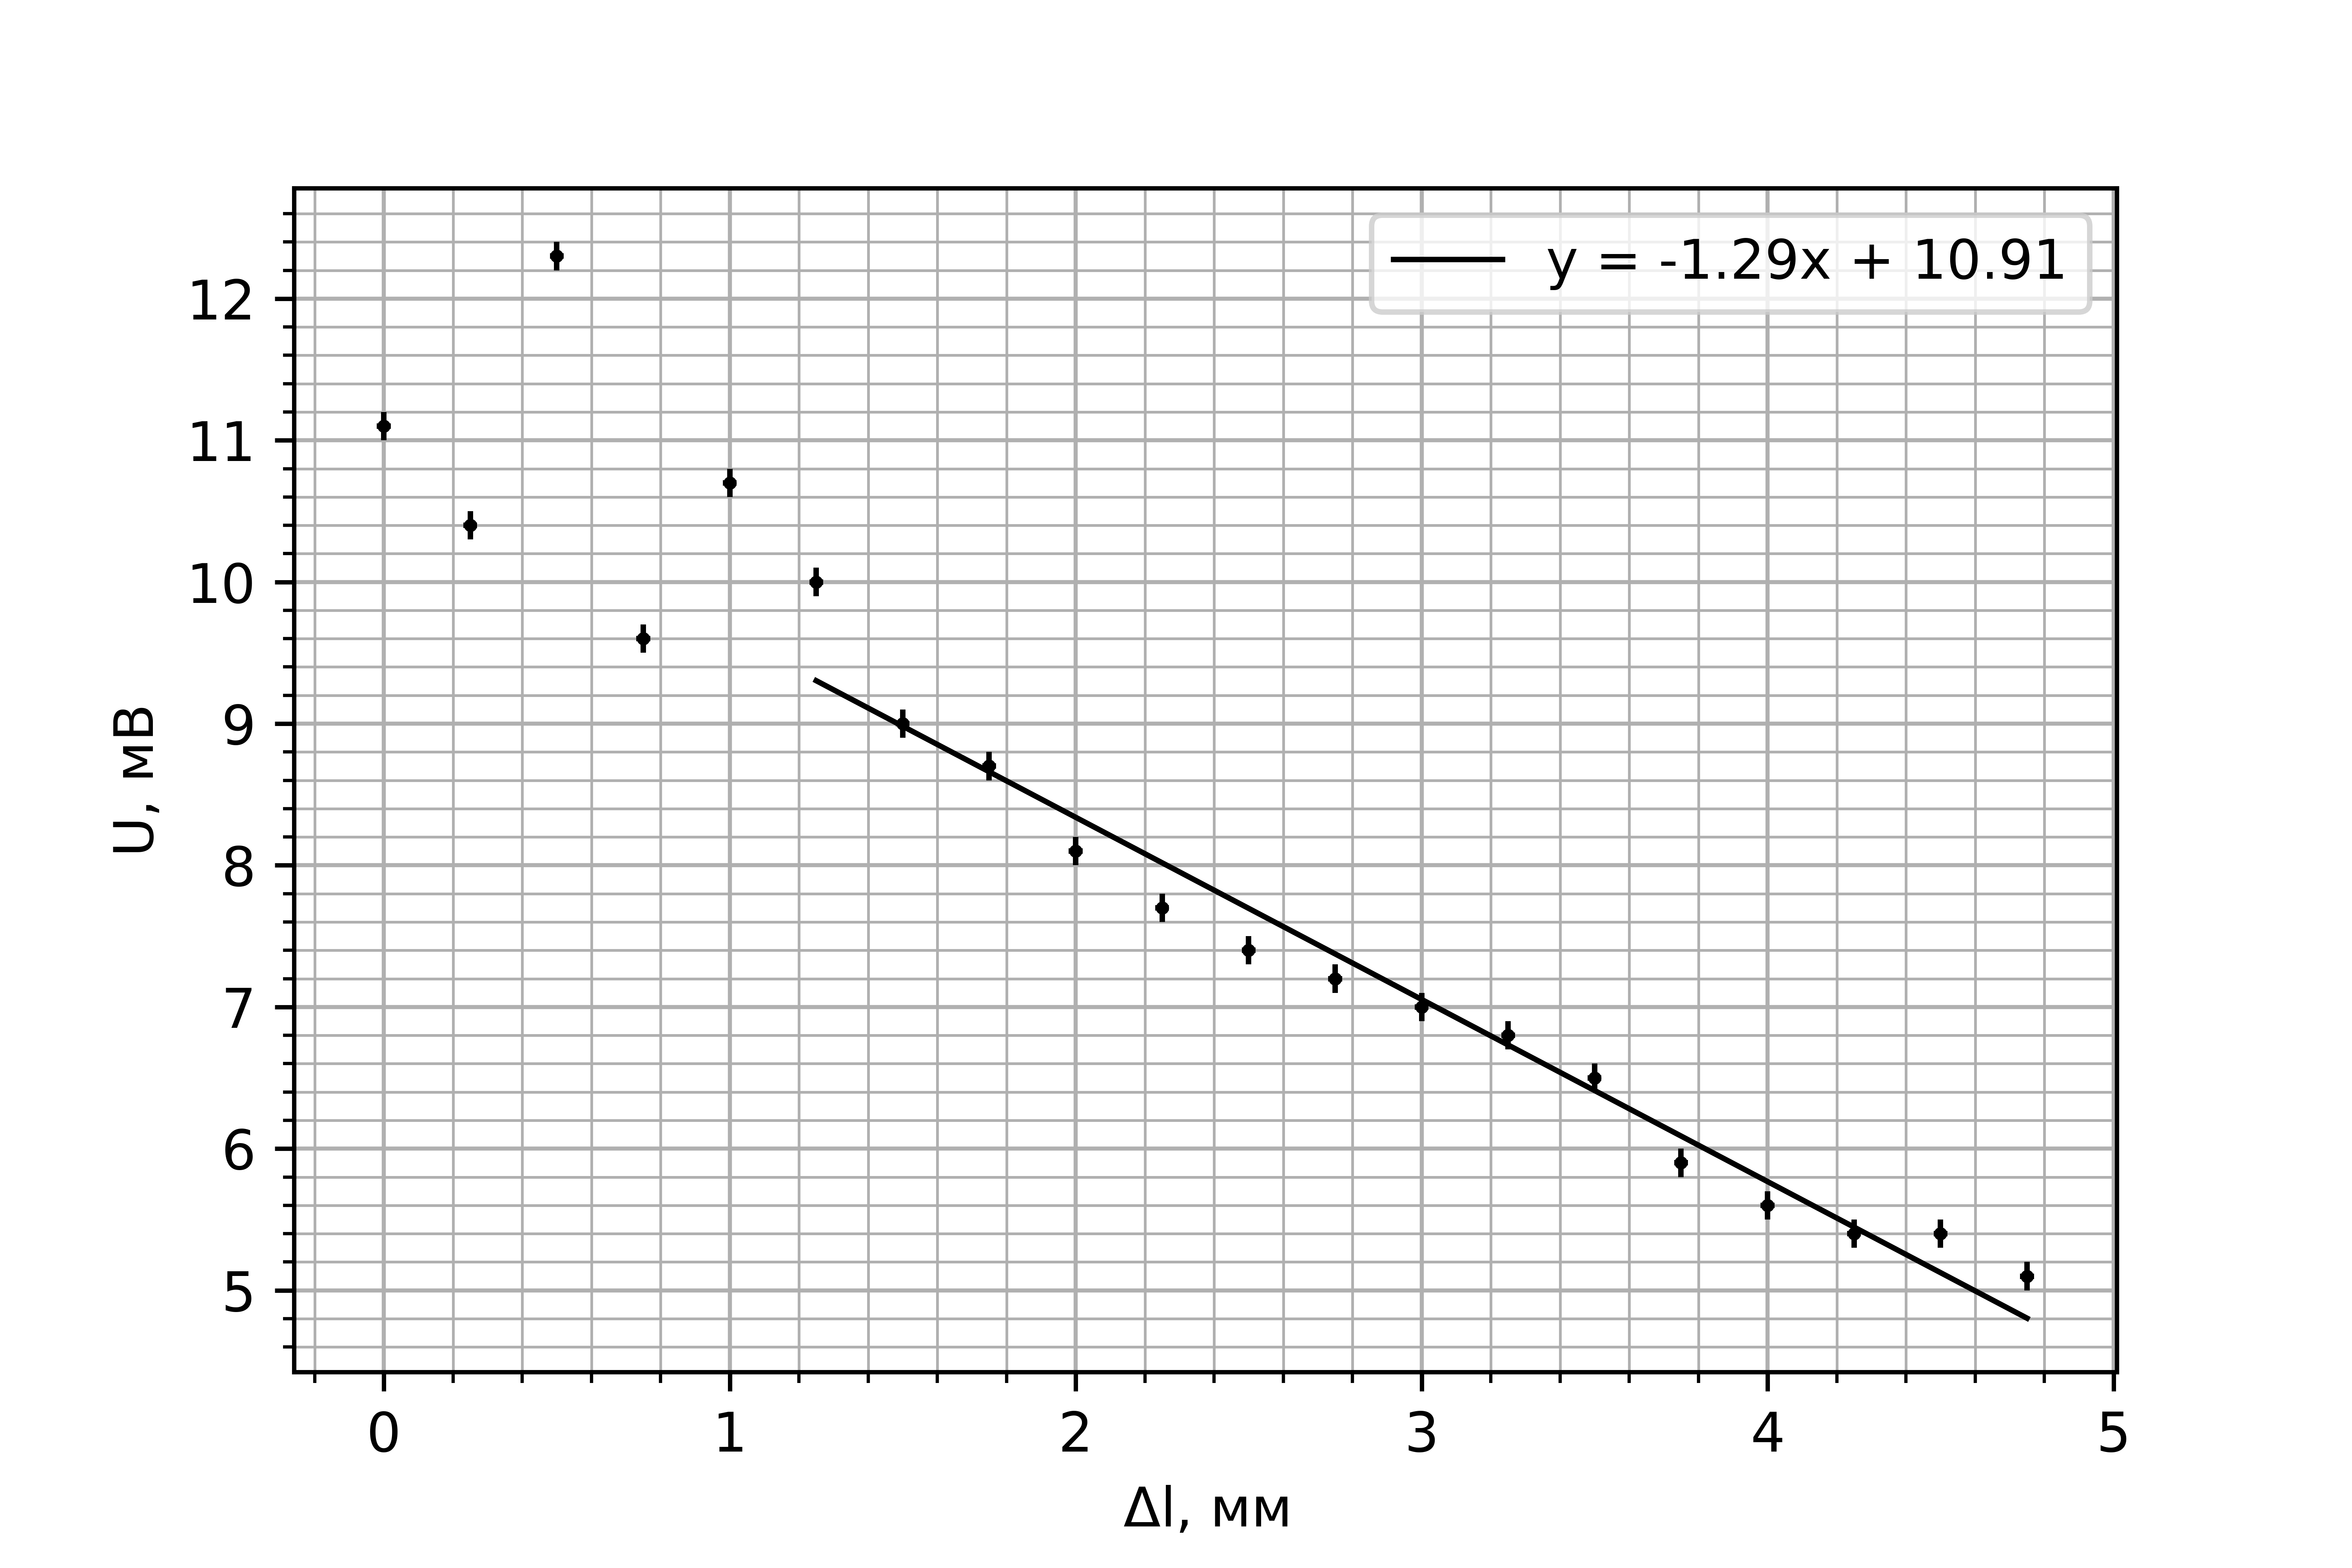
\includegraphics[width=0.87\textwidth]{U(l).png}
    \caption{Зависимость падения напряжения от расстояния между зондами}
    \label{U(l)}
\end{figure}

Из графика найдем коэффициент наклона аппроксимирующей прямой с помощью МНК:
\begin{center}
    k = (-1.29 $\pm$ 0.07) $\frac{\text{мВ}}{\text{мм}}$
\end{center}

Получим значение удельного сопротивления:
\begin{equation*}
    \rho = \frac{kS}{I} = (484 \pm 25) \cdot 10^{-3} \text{ Ом}\cdot{\text{мм}}
\end{equation*}

На графике явно виден участок неоднородности, который может быть объяснен наличием примеси.
Возможные причины неоднородности:
\begin{itemize}
    \item концентрация примеси в выбивающихся точках сильно больше, чем концентрация примеси в остальном полупроводнике
    \item образование собственных точечных дефектов при пластических деформациях
\end{itemize}
Таким образом, приходим к выводу что полупроводник легирован не однородно и/или его кто-то деформировал

\section*{3. Вывод}

В данной работе был изучен двухзондовый метод измерения сопротивления и применен для измерения удельного сопротивления образца, а также найдено удельное сопротивление образца. $\rho= (482 \pm 25)  \cdot 10^{-3} \textup{ Ом}\cdot \textup{мм}$. На основании построенного графика зависимости падения напряжения на участке образца от длины участка был сделан вывод, что образец неоднороден и предложены возможные причины неоднородности: неравномерное распределение концентрации примеси, возможно, пластические деформации.

\end{document}
